\chapter{Responsibility}
\begin{figure}[h]
\centering
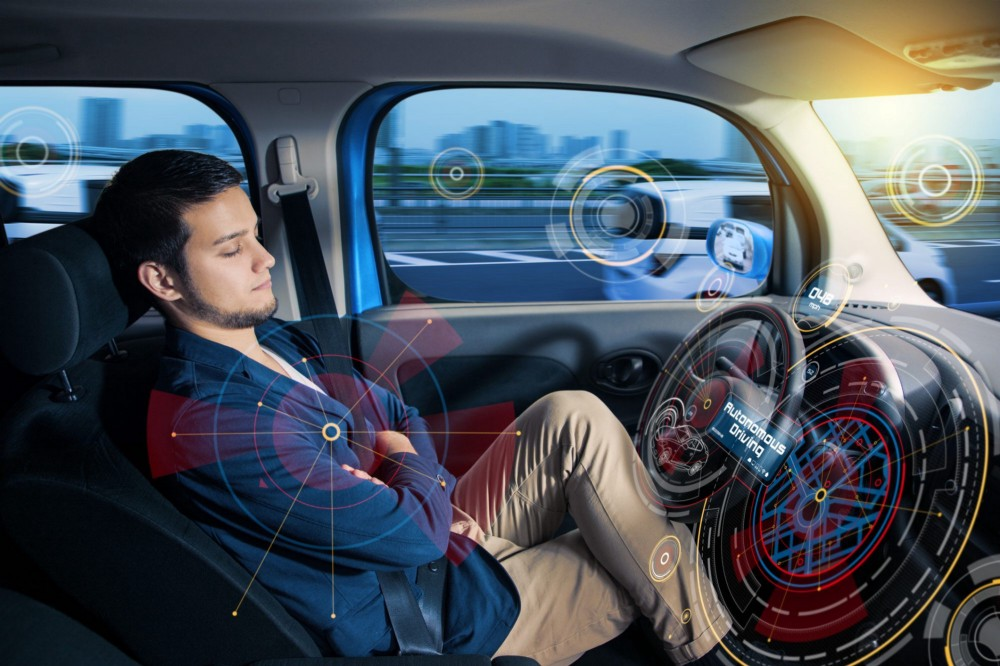
\includegraphics[width=0.8\textwidth]{Capitoli_Report/7.1_Responsibility.png}
\caption{\cite{picresponsibility}}
\label{fig:responsibility}
\end{figure}
\newpage
\section{Introduction}
The case study's objective is to revisit one of the transportation technologies previously discussed in the course through the lens of responsibility theory: the technology we decided to discuss is the \textbf{Intelligent Speed Adaptation} (ISA); it is \textit{a device that automatically limit the speed of a vehicle based on GPS signal or other techniques}. It is advertised that \textbf{its installation can be beneficial for reducing accidents and deaths on the road}.

The two types of responsibility that we think will change the most due to its introduction are \textbf{accountability} and \textbf{moral culpability}.

\emph{(92 words)}

\section{Discussion}
\subsection{Do you think that these changes are problematic? Propose at least two recommendations for improving the responsibility situation.}

We think the introduction of \textbf{ISA} would have effects on the responsibility in terms of \textbf{accountability} and \textbf{moral culpability}. The former is here intended as \textit{"the obligation to explain something that has happened and one's role in its occurrence"}, while the latter means \textit{"being open not only to requests for explanation but also to stronger social and legal responses"}. ISA would ideally be a device that runs continuously in background on the vehicle and so, describing a possible use case, we can consider a situation in which the driver is simply used to going flat-out all the time, letting ISA manage the speed of the car. \textit{But what if ISA fails?}

It could also mean that the driver could be able to overcome the speed limit, without even realizing it. In case this behavior results in the driver hitting a pedestrian, should the \textbf{responsibility} lie with the driver or with the system manufacturer/programmer, who did not manage to produce it as fail proof?

It could be argued that the \textbf{accountability} is totally to be attributed to the driver, who did not respect the limit; but what if he/she was not even realizing his/her wrongdoing, because of the wrong habits of putting all the trust of staying within the limits in the ISA system?

Also, \textbf{culpability} is something that needs to be analysed in the sense that, if the driver is able to use ISA in the way already described, the system is the only barrier that prevents the user from having the undesired behavior of going over the limits. Fallen that barrier, the user is not even realizing what he/she is doing. Both those aspects need to be addressed to define some clear \textit{responsibility boundaries}. One solution can be putting some indicators in the dashboard to inform the driver about the fail of the ISA, or to make it adaptive, so that also the pedal has some feedback to regulate the speed.

\textit{Accountability gaps} could be avoided by the policymaker, that should arrange strict regulation for the production of the ISA. For instance, the manufacturer should provide documentation that simplifies the comprehensibility in case of failures of the device, in order to potentially allocate responsibility also to the producer.

\textit{Culpability gaps} could be avoided ensuring a coordination between the ethical, legal, sociological, and technical field. This could be implemented creating professional profiles characterized by broad-spectrum knowledge in these disciplines, allowing an effective communication between very different contexts and avoiding scapegoating mechanisms.

\emph{(417 words)}
\newpage
\subsection{Would this new situation be helped, in terms of responsibility attribution and/or of institutional organization, by increased collectivization? Why?}
This situation will not be helped by the increased collectivization, because by adding ISA to the car we add a component that is subject to failure: in case of failure, it would be difficult to attribute responsibility to the driver who only trusts the ISA. Why should the vendor, or the mechanic that made the last maintenance, not be considered responsible? And why should they be considered responsible for a failure that they could not forecast, because there were no suspects of an imminent failure during maintenance?

So, adding this component will of course increase collectivization, but it will also reduce the effectiveness of the attribution of responsibility, since it is expanding the audience of possible perpetrators.

\emph{(117 words)}

\emph{(626 words)}

\newpage
\begin{comment}
\begin{thebibliography}{99}

\bibitem [Horizon, 2020]{p1}

Horizon 2020 Commission Expert Group to advise on specific ethical issues raised by driverless mobility (E03659). \textit{Ethics of Connected and Automated Vehicles: recommendations on road safety, privacy, fairness, explainability and responsibility.} Publication Office of the European Union: Luxembourg.

\bibitem [van de Poel, 2015]{p2}

I. van de Poel, L. Royakkers, \& S. D. Zwart (Eds.) (2015) \textit{The problem of many hands.} Moral Responsibility and the Problem of Many Hands (pp. 50–92). Routledge.

\end{thebibliography}
\textit{Document write with \LaTeX. Template founded on Overleaf} (\textbf{Copyright (c) 2020 George Kour}).
\end{comment}